% Load the kaobook class
\documentclass[
    a4paper, % Page size
    fontsize=10pt, % Base font size
    twoside=true, % Use different layouts for even and odd pages (in particular, if twoside=true, the margin column will be always on the outside)
    %open=any, % If twoside=true, uncomment this to force new chapters to start on any page, not only on right (odd) pages
    %chapterentrydots=true, % Uncomment to output dots from the chapter name to the page number in the table of contents
    numbers=noenddot, % Comment to output dots after chapter numbers; the most common values for this option are: enddot, noenddot and auto (see the KOMAScript documentation for an in-depth explanation)
    fontmethod=tex, % Can also use "modern" with XeLaTeX or LuaTex; "tex" is the default for PdfLaTex, and "modern" is the default for those two.
]{kaobook}

% Choose the language
\ifxetexorluatex
    \usepackage{polyglossia}
    \setmainlanguage{english}
\else
    \usepackage[english]{babel} % Load characters and hyphenation
\fi
\usepackage[english=american]{csquotes}  % English quotes

% Load packages for testing
\usepackage{blindtext}
\usepackage{orcidlink}
\usepackage{siunitx}
\usepackage{astro}
% \usepackage{showframe} % Uncomment to show boxes around the text area, margin, header and footer
%\usepackage{showlabels} % Uncomment to output the content of \label commands to the document where they are used

% Load the bibliography package
\usepackage[backend=biber, style=numeric-comp,backref, sorting=none, firstinits=true]{biblatex} 
\DeclareSourcemap{
 \maps[datatype=bibtex,overwrite=true]{
  \map{
    \step[fieldsource=Collaboration, final=true]
    \step[fieldset=usera, origfieldval, final=true]
  }
 }
}

\renewbibmacro*{author}{%
  \iffieldundef{usera}{%
    \printnames{author}%
  }{%
    \printfield{usera}, \printnames{author}%
  }%
}%

\usepackage{kaobiblio}
% \bibliographystyle{apsrev4-2}
\addbibresource{thesis.bib} % Bibliography file

% Load mathematical packages for theorems and related environments
\usepackage[framed=true]{kaotheorems}

% Load the package for hyperreferences
\usepackage{kaorefs}

\graphicspath{{figures/}{images/}} % Paths where images are looked for

\makeindex[columns=3, title=Alphabetical Index, intoc] % Make LaTeX produce the files required to compile the index


\begin{document}

%----------------------------------------------------------------------------------------
%   BOOK INFORMATION
%----------------------------------------------------------------------------------------
\subject{Doctoral Thesis}
% \titlehead{Optical Follow-Up of High-Energy Neutrinos}
\title[Optical Follow-Up of High-Energy Neutrinos]{Optical Follow-Up of High-Energy Neutrinos}
\author[SR]{Simeon Reusch}% \orcidlink{0000-0002-7788-628X}}
\date{\today}
\publishers{Humboldt-Universität zu Berlin}

%----------------------------------------------------------------------------------------

\frontmatter % Denotes the start of the pre-document content, uses roman numerals

%----------------------------------------------------------------------------------------
%   COPYRIGHT PAGE
%----------------------------------------------------------------------------------------

\makeatletter
\uppertitleback{\@titlehead} % Header

\lowertitleback{
    % \textbf{Disclaimer} \\
    % You can edit this page to suit your needs. For instance, here we have a no copyright statement, a colophon and some other information. This page is based on the corresponding page of Ken Arroyo Ohori's thesis, with minimal changes.
    
    % \medskip
    
    \textbf{Copyright} \\
    \cczero\ This book is released into the public domain using the CC0 code. To the extent possible under law, I waive all copyright and related or neighbouring rights to this work. To view a copy of the CC0 code, visit: \\\url{http://creativecommons.org/publicdomain/zero/1.0}
    
    \medskip
 
    This thesis was typeset with the help of \href{https://sourceforge.net/projects/koma-script}{\KOMAScript} and \href{https://www.latex-project.org}{\LaTeX} using the \href{https://github.com/fmarotta/kaobook}{kaobook} class.
    
    \medskip

    The code used to typeset this thesis and create the figures within can be accessed at \href{https://github.com/simeonreusch/koma-thesis}{github.com/simeonreusch/thesis}

    \medskip
    
    \textbf{Publisher} \\
    First published in August 2023 by \@publishers
}
\makeatother


\maketitle

%----------------------------------------------------------------------------------------
%   PREFACE
%----------------------------------------------------------------------------------------

% \chapter*{Preface}

% \blindtext

%----------------------------------------------------------------------------------------
%   TABLE OF CONTENTS & LIST OF FIGURES/TABLES
%----------------------------------------------------------------------------------------

\begingroup % Local scope for the following commands

% Define the style for the TOC, LOF, and LOT
%\setstretch{1} % Uncomment to modify line spacing in the ToC
%\hypersetup{linkcolor=blue} % Uncomment to set the colour of links in the ToC
\setlength{\textheight}{230\vscale} % Manually adjust the height of the ToC pages

% Turn on compatibility mode for the etoc package
%\etocstandarddisplaystyle % "toc display" as if etoc was not loaded
%\etocstandardlines % "toc lines as if etoc was not loaded

\tableofcontents % Output the table of contents

\listoffigures % Output the list of figures

% Comment both of the following lines to have the LOF and the LOT on different pages
\let\cleardoublepage\bigskip
\let\clearpage\bigskip

\listoftables % Output the list of tables

\endgroup

\mainmatter
\setchapterstyle{kao}

%\chapter{Theoretical background}
%\addpart{Title of the Part}
\pagelayout{margin} % Restore margins
\setchapterimage[7cm]{ic_icecube.jpg}
\chapter{The IceCube Detector}
\labch{IceCube}
One of the two most relevant instruments for this thesis is the \textit{IceCube Detector}, a neutrino detector located at the geographic South Pole. It is the successor to the Antarctic Muon And Neutrino Detector Array (AMANDA) at the same location \sidecite{Andres1999, Andres2000}. 
\begin{marginfigure}
    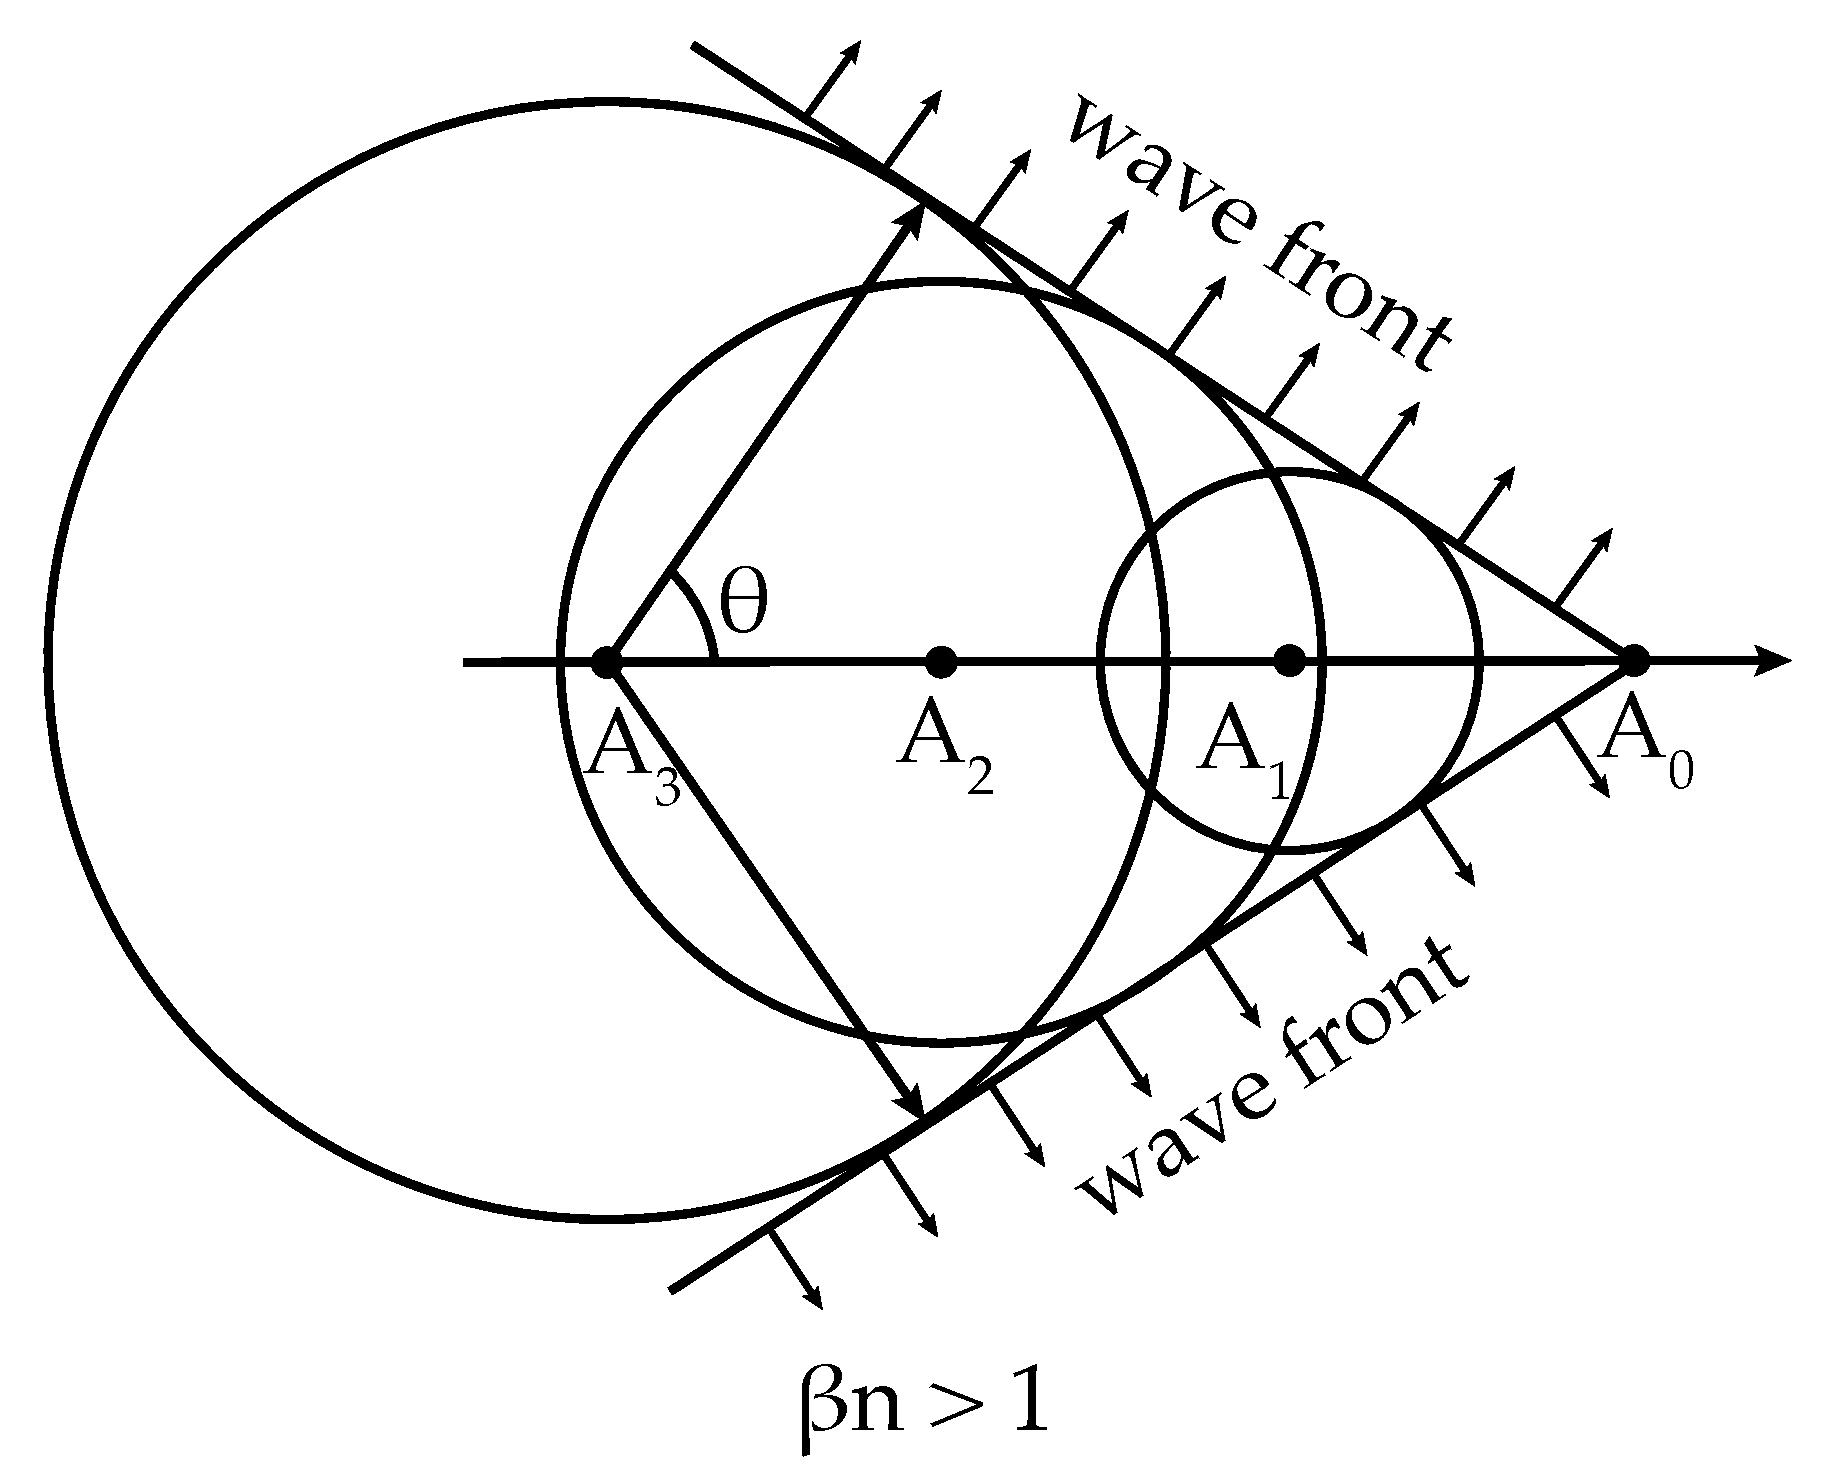
\includegraphics{ic_cherenkov1.png}
    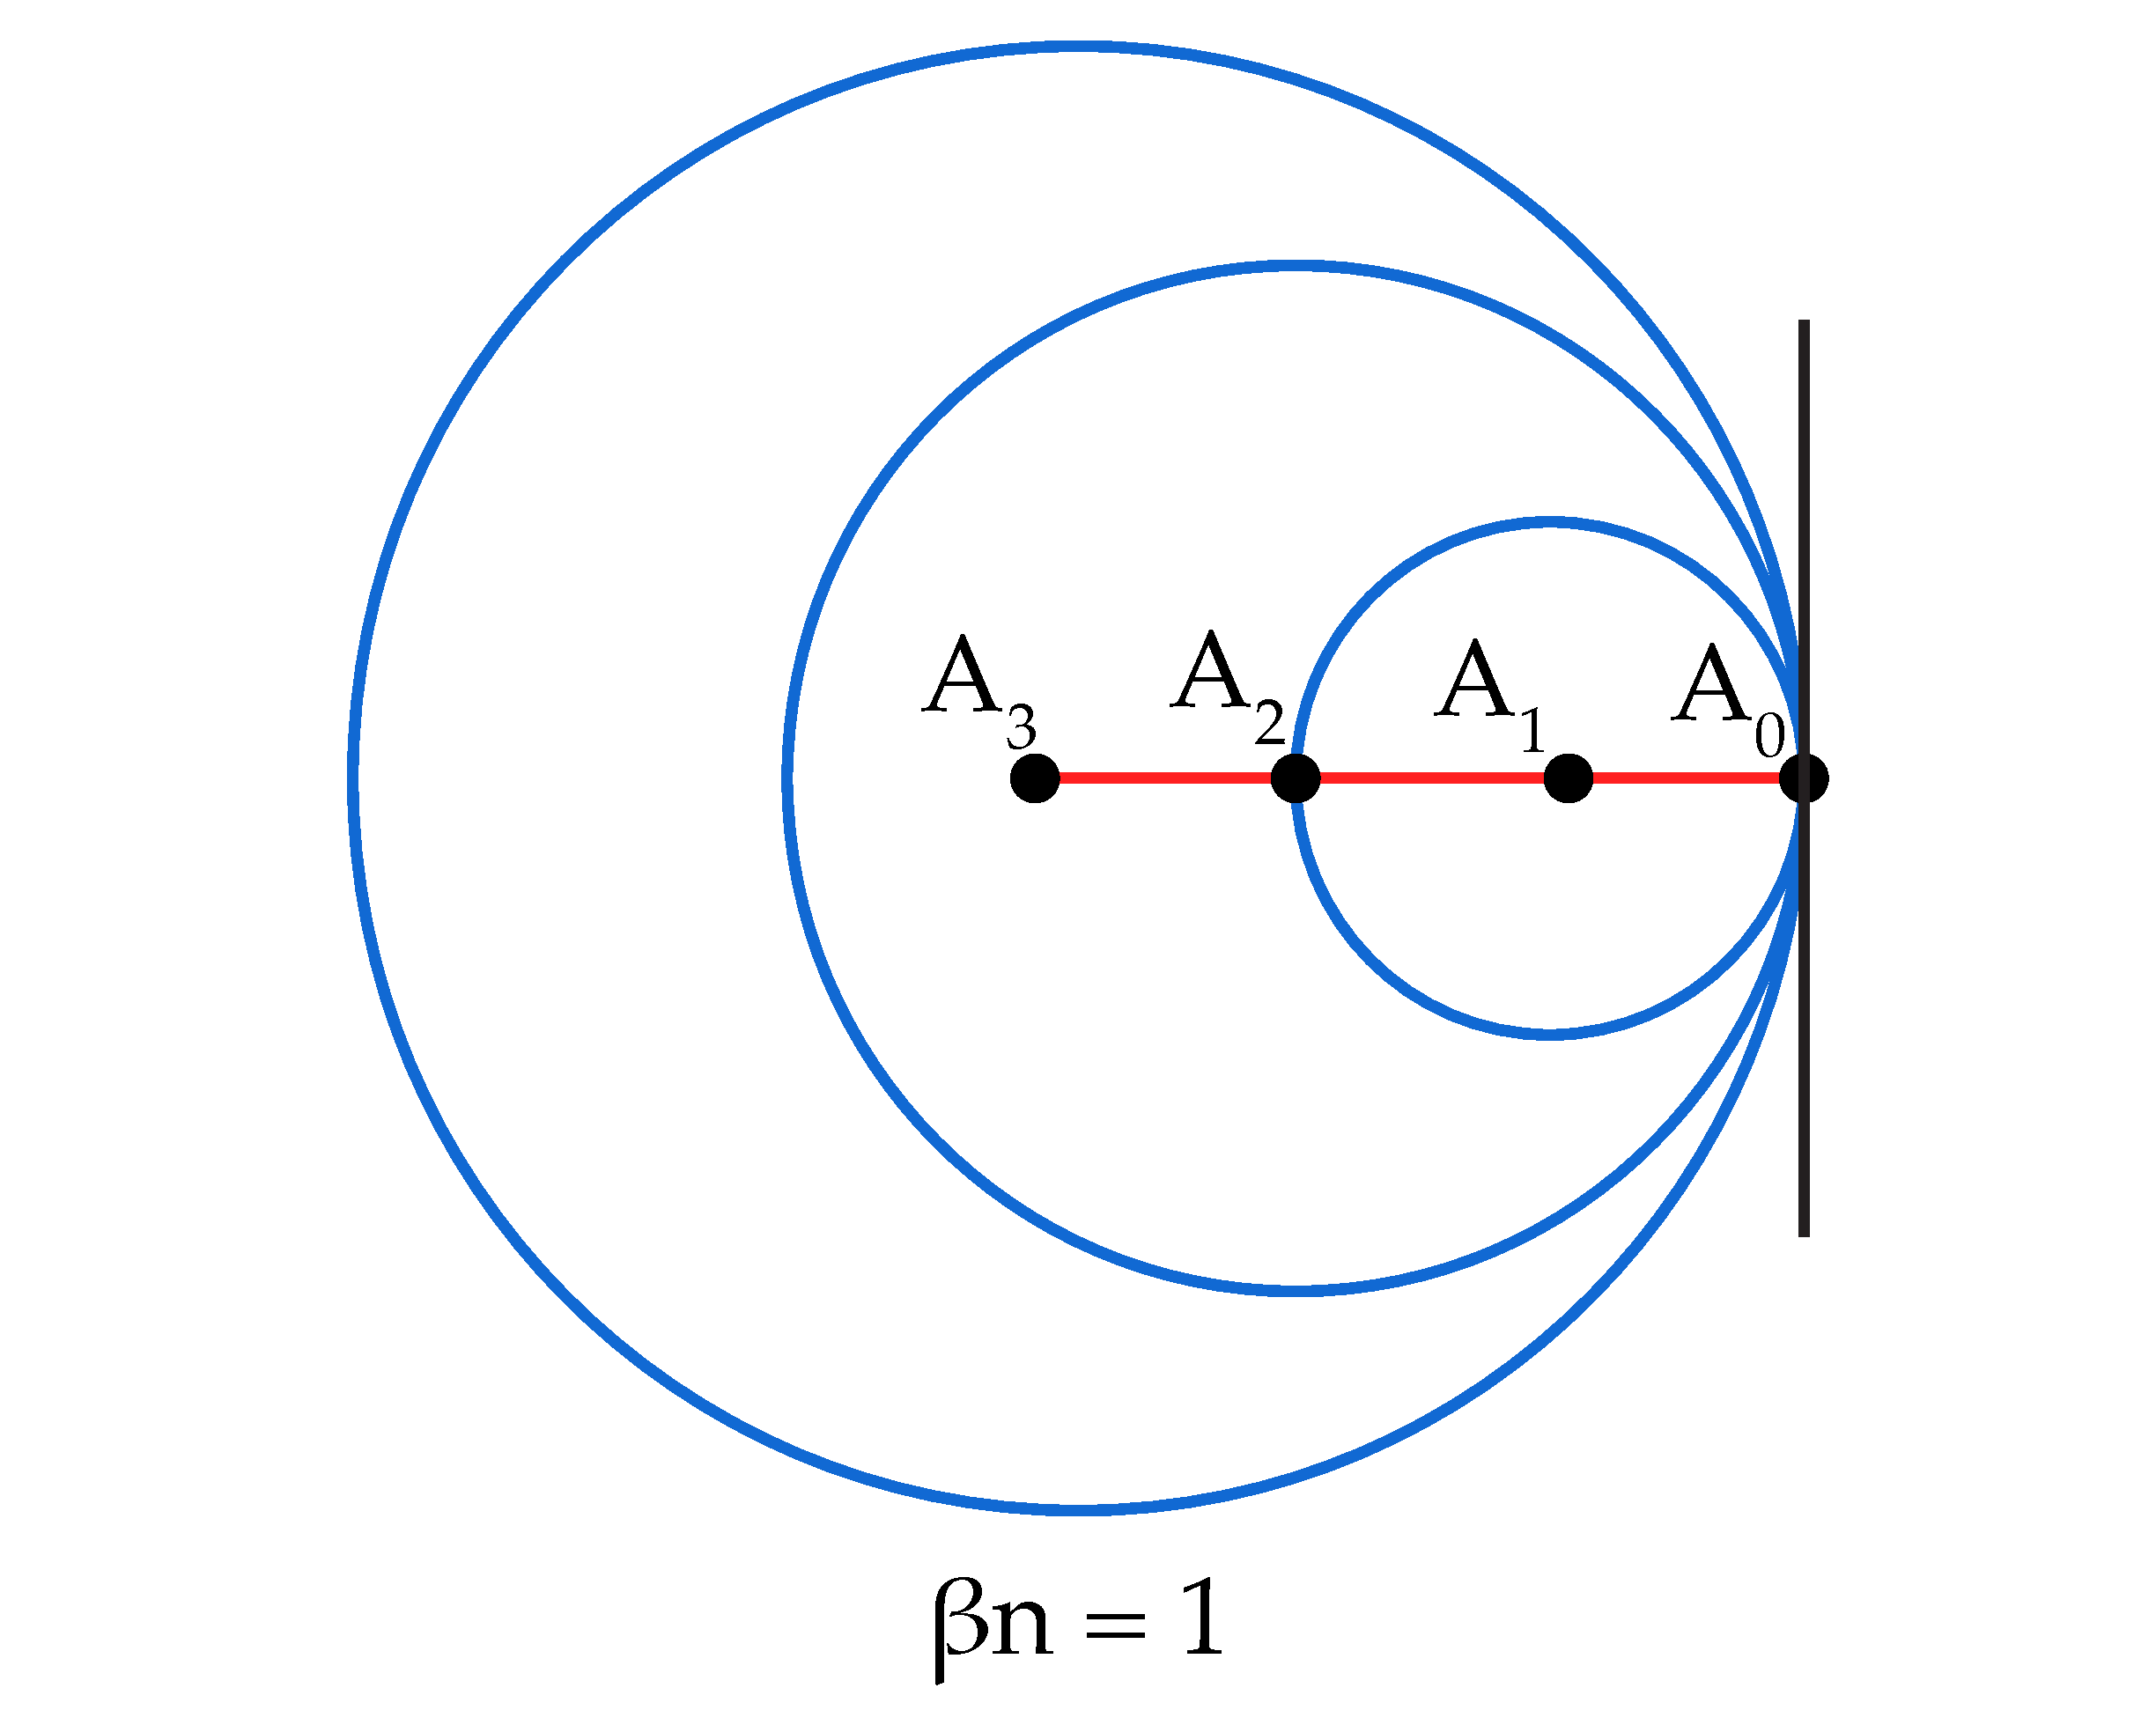
\includegraphics{ic_cherenkov2.png}
    \caption[Cherenkov radiation]{The principle of Cherenkov radiation. In the upper figure (A) Cherenkov radiation is emitted, as the radiation emitted at different points in time forms mutual wavefronts. In the figure on the bottom (B), all radiation is cancelled out by destructive interference (all circles are subsets of the first on the left, as the particle is not moving faster than light in the medium). From \cite{LAnnunziata2020}.}
    \labfig{cherenkov}
\end{marginfigure}
The basic oeprational principle of IceCube (and already of AMANDA) is the detection of Cherenkov light within the antarctic ice. When charged secondary particles created by neutrino interactions travel through the ice, their speed exceeds the phase velocity of light in ice and they emit Cherenkov radiation. The detector consists of 5160 individual digital optical modules (DOMs), buried deep in the ice. These are sensitive to the Cherenkov radiation.

\section{Cherenkov radiation} \label{cherenkov_radiation}

Cherenkov radation was first detected in 1934 by Soviet scientist Pavel Cherenkov \sidecite{Cherenkov1934}. It occurs when charged particles travel within a medium with a velocity exceeding the speed of light in that medium. The refractive index in a medium is defined as $n=\frac{c_0}{c_m}$, where $c_m$ is the speed of light in vacuum and $c_m$ is the phase velocity of light in that medium. Note that the phase velocity of light in a medium can exceed $c_0$, so $n<1$ is possible. 

When charged particles cross an electrically neutral dielectric medium, atoms along the particle's path are briefly polarized and emit electromagnetic radiation. 

For slow particles, this radiation destructively interferes with itself, canceling out all signals (see the bottom panel of Fig. \ref{fig:cherenkov}). Now, if the particle is travelling faster than speed of light within the medium $c_m$, this destructive interference does not happen. Rather, a cone-shaped wavefront gets created (see top panel of Fig. \ref{fig:cherenkov}). This wavefront constitutes Cherenkov radiation. If the particle has speed $v=\beta c_0$, the angle $\theta$ between the particle trajectory and the direction of the Cherenkov radiation can be calculated as \sidecite{LAnnunziata2020}:

\begin{equation}
\cos{\theta} = \frac{\beta}{n}
\end{equation}

For example: If the medium is ice, to first order the refractive index $n\approx1.31$.\sidenote{This is of course rather crude. The $n$ of Antarctic glacial ice depends e.g. on depth; a fact we will come back to later when discussing directional reconstruction of high-energy IceCube neutrinos.} A secondary muon traveling through the ice at $0.999\,c_0$ will therefore emit Cherenkov light at an angle of $\theta = \cos^{-1}{\big(\frac{0.999}{1.31}\big)} \approx \SI{40}{\degree}$. 
\begin{marginfigure}
    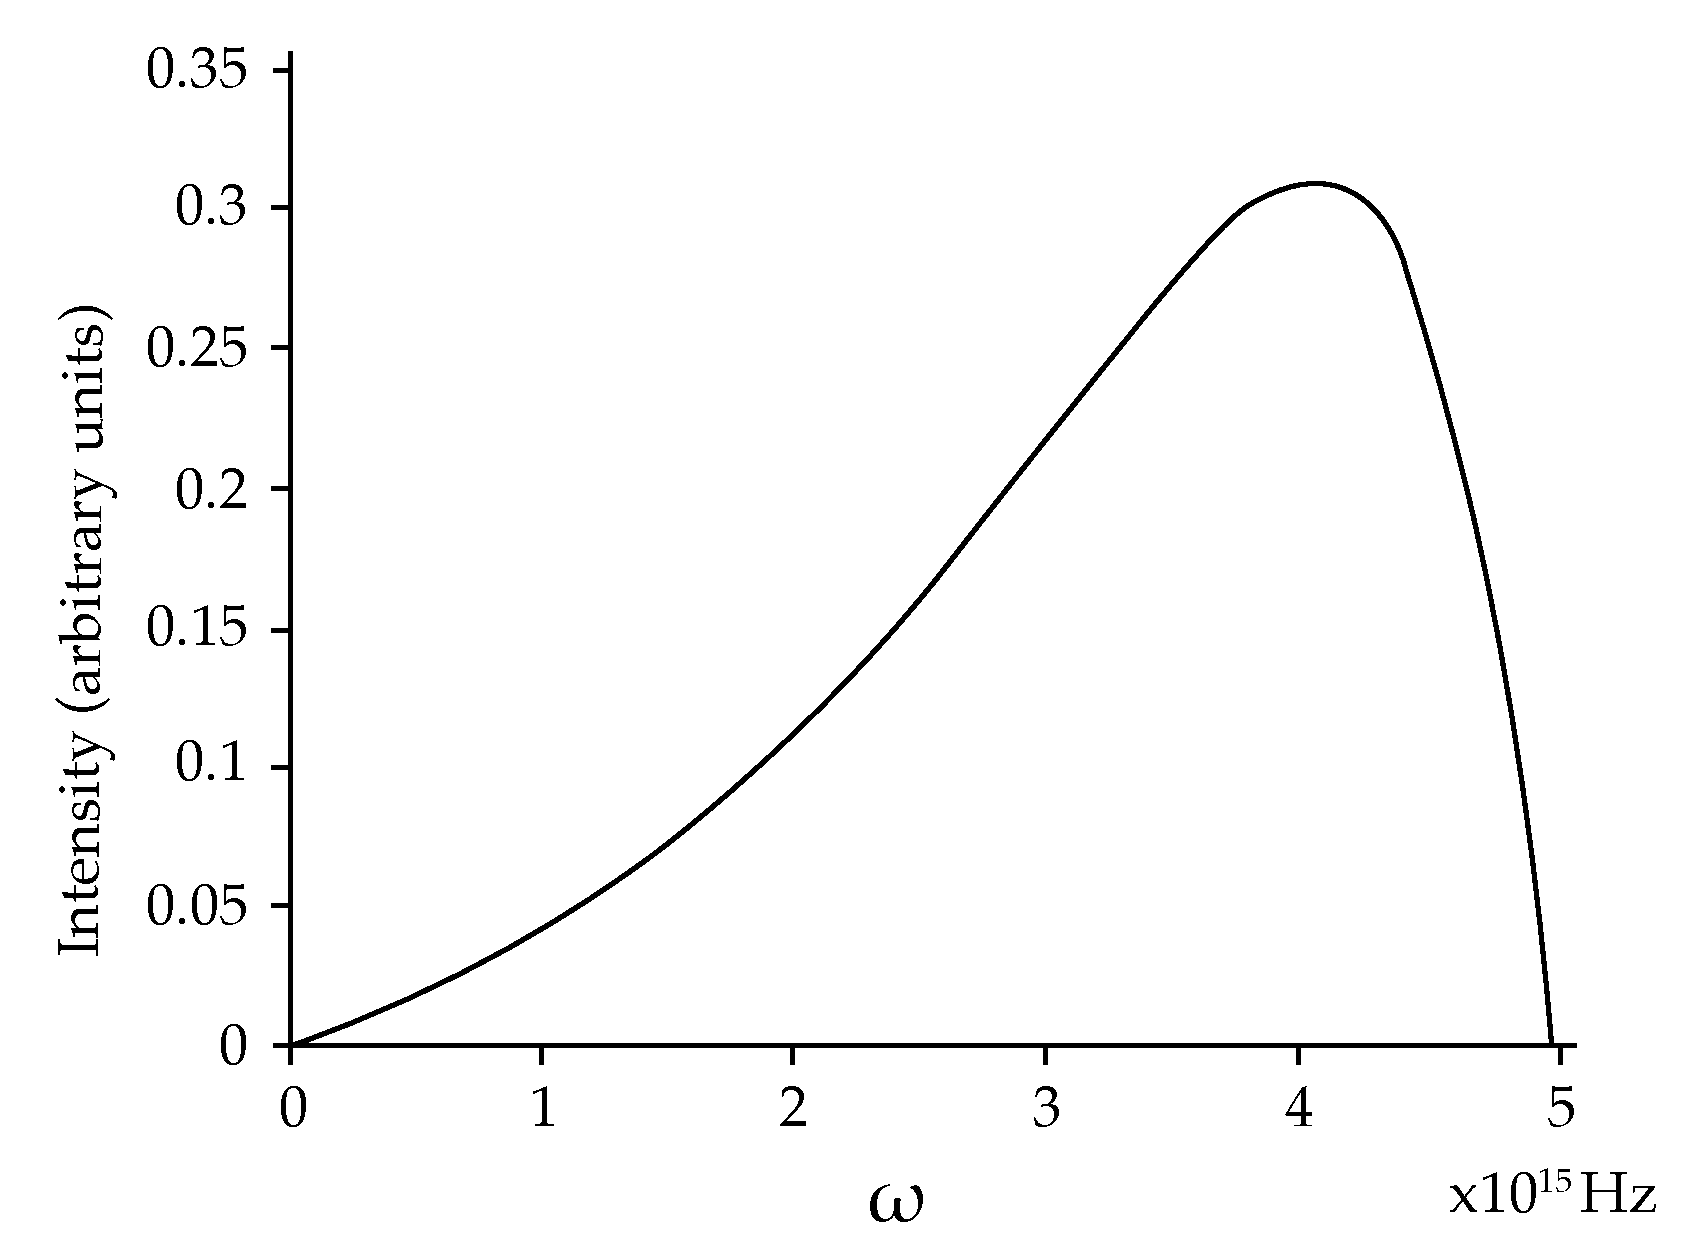
\includegraphics{ic_cherenkov_spectrum.png}
    \caption[Cherenkov spectrum]{Cherenkov spectrum for a particle with $v=0.8 \,c_0$ in water. The intensity peaks at $\SI{4e15}{\Hz}$, corresponding to a wavelength of \SI{75}{\nm}, lying at the high-frequency end of the UV spectrum. From \cite{Fulop1992}.}
    \labfig{cherenkov_spectrum}
\end{marginfigure}
Cherenkov radiation does not have spectral peaks, but is continuous, with a relative intensity proportional to the frequency. Note that the refractive index of a medium is also frequency dependent, dropping below 1 in the X-ray. From this it follows that Cherenkov radiation appears blue to the human eye (the high-frequency part dominates) and peaks in the ultra violet (UV), before it sharply drops off in the X-ray regime \sidecite{Fulop1992}, see Fig. \ref{fig:cherenkov_spectrum}.

\section{IceCube instrumentation}

IceCube detects neutrinos by observing the optical part of their secondary particle Cherenkov spectrum (see section \ref{cherenkov_radiation} above). To understand how this is done, one first needs to look at the working principe of a photomultiplier tube (PMT).

\subsection*{Photomultiplier tubes}
A PMT is a device used to detect very faint light signals by amplifying them. They consist of vacuum tubes and were successfully realized for the first time in the 1930s \sidecite{Iams1935}.

\begin{figure}[h!]
    \includegraphics{ic_pmt.png}
    \caption[PMT schematic]{A photomultiplier tube. From \cite{Bednarski2014}.}
    \labfig{pmt}
\end{figure}

As one can see in Fig. \ref{fig:pmt}, there are three principal components: a \textit{cathode}, a number of \textit{dynodes} and an \textit{anode}. When photons hit the cathode, they can release electrons via the photoelectric effect \sidecite{Einstein1905}. These photoelectrons are then accelerated (towards the right side in Fig. \ref{fig:pmt}) by an electric field within the tube. This field is generated by applying a high voltage between the cathode and the anode.

To amplify the signal, a number of dynodes is placed in between. These are additional electrodes with subsequently higher voltages. When the photoelectron hits the first dynode, a number of secondary electrons are generated, which are subsequently accelerated towards the next dynode by the electric field. This process repeats for every dynode, generating an avalanche of electrons amplifying the original single photoelectron signal by a large factor.

\subsection*{Detector layout}
Fig. \ref{fig:ic_sideon} shows the detector side-on, while Fig. \ref{fig:ic_top_down} shows a top-down view.
\begin{marginfigure}
    \includegraphics{ic_side_view.png}
    \caption[IceCube side-on]{Side view of the IceCube detector, showing the instrumented array deep in the antarctic glacial ice. In the center on top is the IceCube Laboratory, were data acquisition takes place. From \cite{Ahlers2018a}.}
    \labfig{ic_sideon}
\end{marginfigure}
\begin{marginfigure}
    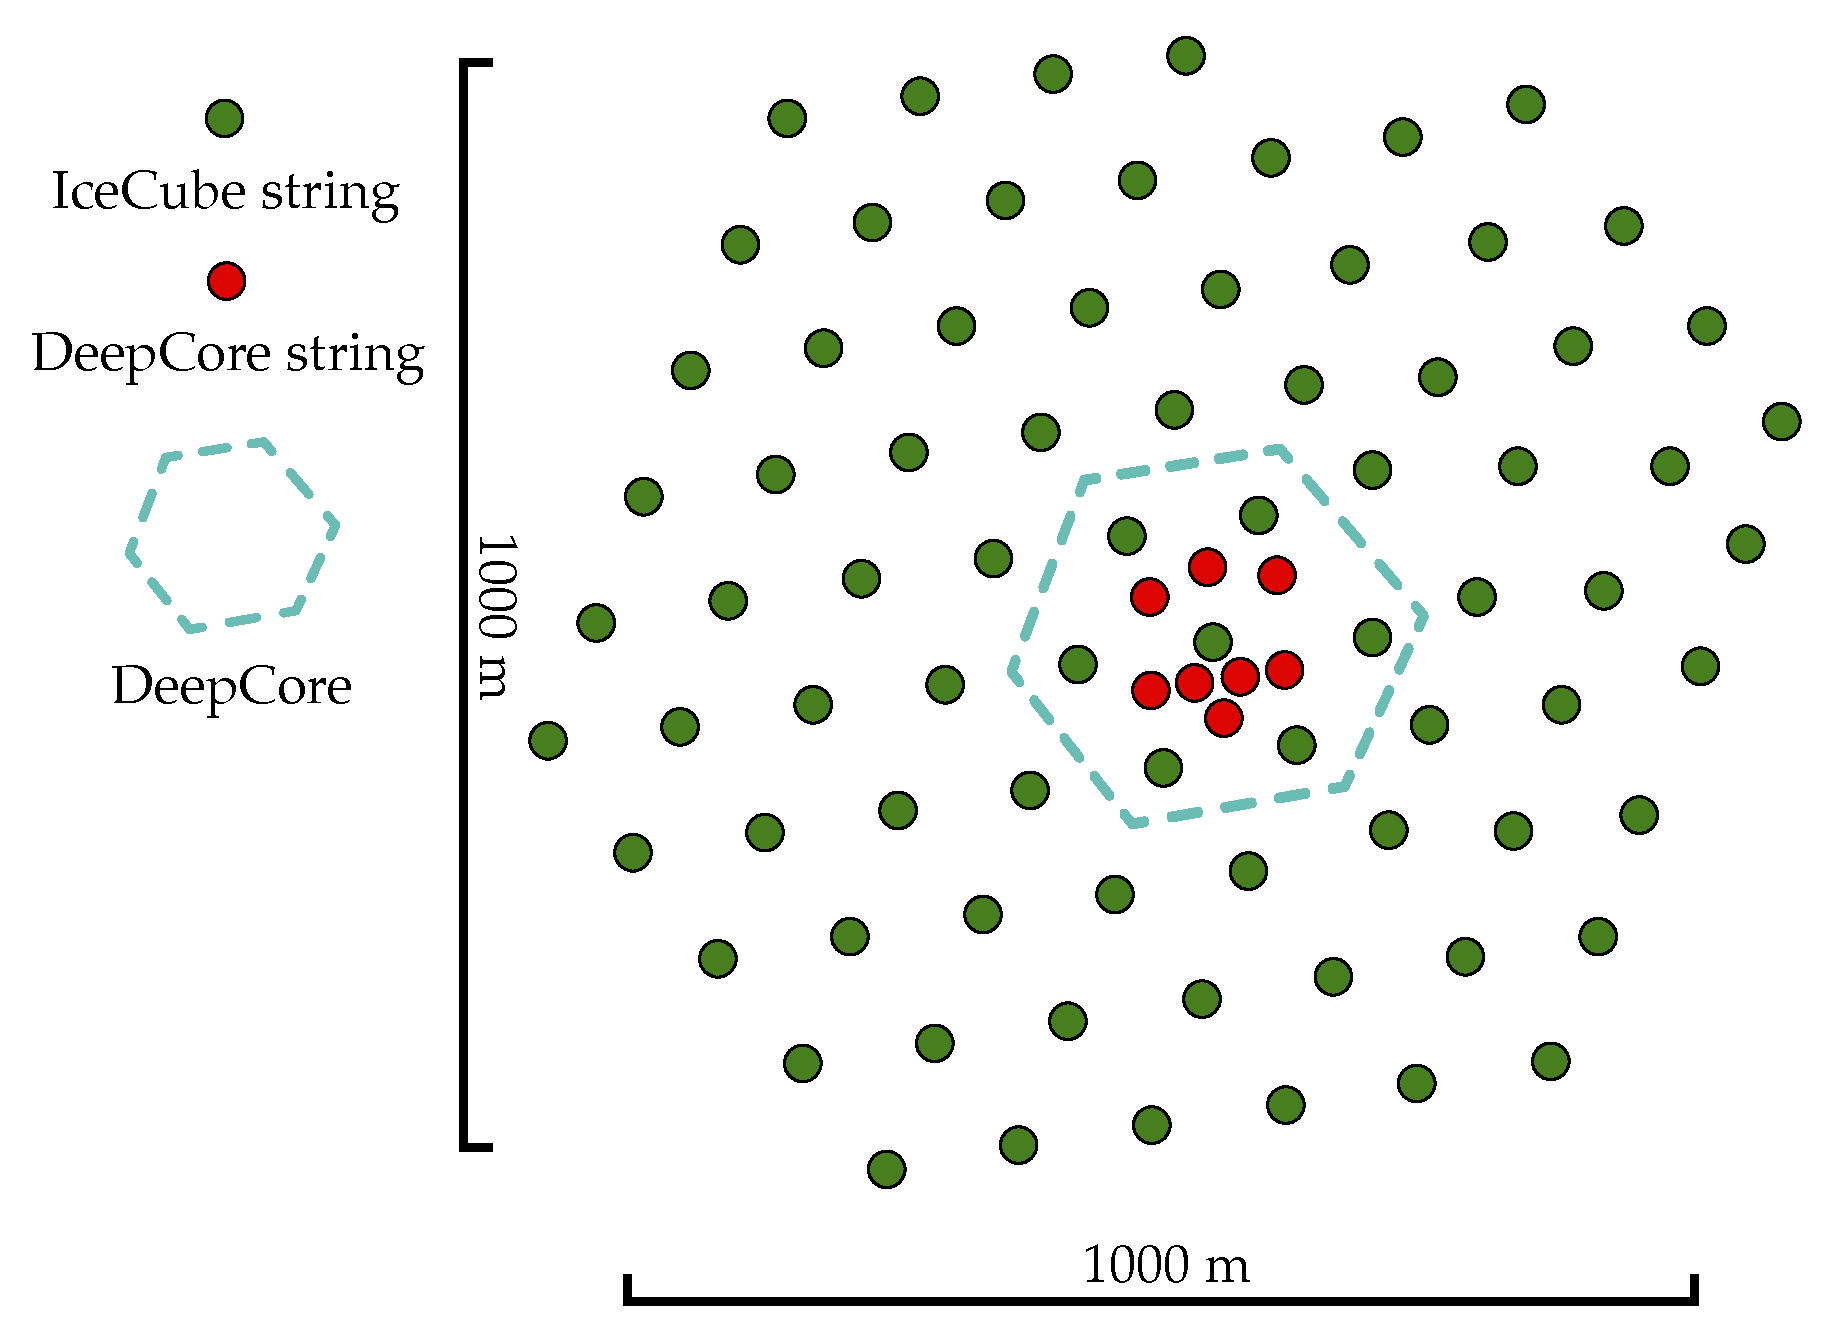
\includegraphics{ic_top_view.png}
    \caption[IceCube top-down view]{Top-down view of the IceCube detector, spanning \SI{1}{\square\km} on the surface. From \cite{Ahlers2018a}.}
    \labfig{ic_top_down}
\end{marginfigure}


\setchapterimage[7cm]{ztf_telescope.png} % Optionally specify the height
\setchapterpreamble[u]{\margintoc}
\chapter{The Zwicky Transient Facility}
\labch{ZTF}
The second instrument relevant for this thesis is the Zwicky Transient Facility (ZTF). Named after the notorious Swiss-American astronomer Fritz Zwicky, it is a wide-field optical survey telescope located at Mount Palomar in California, United States, at 1700 m above sea level.\marginnote{See \url{https://sites.astro.caltech.edu/palomar/about/telescopes/oschin.html} for a historical overview.} The housing, the 1.22 m (48 inch) Samuel Oschin telescope, is a Schmidt design and was inaugurated in 1948 \cite{Harrington1952}. Originally, the telescope used photographic plates. As these have obvious drawbacks, and because technological progress made it possible, the Near-Earth Asteroid Tracking (NEAT) program \cite{Pravdo1999} replaced the photographic plates with a charge-coupled device (CCD) camera in the early 2000s.

The camera was updated several times over the course of the next years. The immediate predecessor of ZTF, the Palomar Transient Factory (PTF) \cite{Law2009}, began operation in 2009. Equipped with a 96 Megapixel camera, it already had many of the characteristics of ZTF: A fully automated survey, searching for optical transients.

PTF's successor in spirit, ZTF, was the first electronic camera using almost the full field of view (FOV) of the P48. The main design metric for ZTF was \textit{volumentric survey speed} \cite{Bellm2016}. This is the volume within which an object of given absolute magnitude can be detected in one exposure, divided by the total time for the exposure (observation plus overhead). The system saw first light in 2017, and started its scientific use in the year after. As of writing, it is still operational.

\section{Telescope Design}
A Schmidt telescope is 

\section{Camera}

\section{Image Processing}



%\chapter{The ZTF neutrino follow-up program}
%\chapter{Candidate TDE AT2019fdr: a possible source?}
%\chapter{The ZTF nuclear sample}
%\chapter{Conclusion and Outlook}
\appendix

\pagelayout{wide} % No margins
\addpart{Appendix}
\pagelayout{margin} % Restore margins


%----------------------------------------------------------------------------------------

\backmatter % Denotes the end of the main document content
\setchapterstyle{plain} % Output plain chapters from this point onwards

%----------------------------------------------------------------------------------------
%   BIBLIOGRAPHY
%----------------------------------------------------------------------------------------

% The bibliography needs to be compiled with biber using your LaTeX editor, or on the command line with 'biber main' from the template directory
%\defbibnote{bibnote}{Here are the references in citation order.\par\bigskip} % Prepend this text to the bibliography
\printbibliography[heading=bibintoc, title=Bibliography] % Add the bibliography heading to the ToC, set the title of the bibliography and output the bibliography note

%----------------------------------------------------------------------------------------
%   INDEX
%----------------------------------------------------------------------------------------

% The index needs to be compiled on the command line with 'makeindex main' from the template directory

\printindex % Output the index

\end{document}
